\documentclass[10pt,a4paper]{article}
\usepackage[a4paper,left=16mm,right=16mm,top=19mm,bottom=18mm,headheight=12pt,headsep=7mm,footskip=11mm]{geometry}
\usepackage[T1]{fontenc}
\usepackage[utf8]{inputenc}
\usepackage{lmodern}
\usepackage{amsmath,amssymb,graphicx,booktabs,pdflscape,caption}
\usepackage{float,multicol,titlesec,fancyhdr,microtype}
\usepackage{xurl}
\usepackage[hidelinks]{hyperref}
\urlstyle{same}
\pagestyle{fancy}
\fancyhf{}
\fancyhead[L]{\fontsize{8}{10}\selectfont LSGI2802\enspace |\enspace Assignment 2}
\fancyfoot[C]{\thepage}
\renewcommand{\headrulewidth}{0pt}
\renewcommand{\footrulewidth}{0pt}
\setlength{\parindent}{0pt}
\setlength{\parskip}{3pt}
\linespread{1.03}
\setlength{\columnsep}{8mm}
\setlength{\multicolsep}{6pt}
\raggedcolumns
\raggedbottom
\emergencystretch=2em
\clubpenalty=10000
\widowpenalty=10000
\interlinepenalty=150
\titleformat{\section}{\fontsize{11}{13}\selectfont\bfseries}{}{0pt}{}
\titlespacing*{\section}{0pt}{8pt}{4pt}
\captionsetup{font=small,labelfont=bf,labelsep=period,justification=raggedright,singlelinecheck=false,skip=7pt}
\setlength{\intextsep}{8pt}
\setlength{\textfloatsep}{9pt}
\setlength{\floatsep}{9pt}
\hypersetup{pdfsubject={LSGI2802 Assignment 2},pdfauthor={ZHANG Shizhuo}}
\begin{document}

{\fontsize{22}{25}\selectfont\bfseries\raggedright
Beyond the 15-minute threshold: measuring walking access to primary care in Hong Kong\par}
{\small ZHANG Shizhuo\par}
\vspace{7pt}

{\fontsize{11}{14}\selectfont
\textbf{Abstract}\par\vspace{3pt}
Neighbourhoods with no clinic within a 15-minute walk receive the same zero opportunity count, although journeys to care may differ considerably~\cite{moreno2021,tomasiello2023}. We examine what this classification conceals in walking access to public primary care in Hong Kong. The analysis compares minimum travel time, clinics reachable within 15 minutes and gravity-based accessibility, which discounts clinics as travel time increases. Of 284 neighbourhood proxy locations, 172 have no clinic within 15 minutes. Within this group, nearest-clinic times and access to more distant alternatives vary despite broadly similar spatial patterns across the measures. Slower walking reduces accessible opportunities even where neighbourhood rankings remain stable. Gravity-based accessibility describes potential clinic choice, while minimum travel time indicates the journey needed to reach the nearest clinic. Assessing both helps distinguish limited nearby choice from long journeys and provides a basis for incorporating walking ability and route conditions.\par}
\vspace{5pt}

\begin{multicols}{2}
\section*{Introduction}
Spatial access to primary care depends on proximity to providers and the availability of services. Hong Kong research has assessed these dimensions using nearest-provider and supply--demand measures~\cite{xiong2022}. The 15-minute-city framework offers a clear planning benchmark for local access~\cite{moreno2021}.

Cumulative opportunity estimates depend on the travel-time threshold~\cite{tomasiello2023}. A 15-minute clinic count gives the same zero score whether the nearest clinic lies just beyond the threshold or requires a much longer journey. It also excludes alternatives beyond that boundary. Agreement between accessibility maps may therefore conceal differences among poorly served locations.

We compare minimum travel time, cumulative opportunities and gravity-based accessibility to public primary care across Hong Kong. Using the same neighbourhood proxy origins and three-dimensional pedestrian network, we assess low-access classifications, differences among zero-opportunity locations and sensitivity to slower walking.

\section*{Methods}
Clinic locations, census data and the pedestrian network came from CSDI, retrieved on 24 October 2026~\cite{csdiClinics,csdiTPU,csdiCensus,csdiNetwork}. We merged co-located records and applied consultation hours for an ordinary Monday at 15:00, retaining 74 equally weighted clinic sites. Population-density rankings of census polygons guided outdoor-network proxy selection in 284 of 292 Tertiary Planning Units (TPUs); eight remained unresolved.

Routing retained enabled links outside paid areas, preserving elevation, direction and opening schedules. Walking speed was 4.8~km\,h$^{-1}$ and lift speed 60~m\,min$^{-1}$, without waiting. Clinic connector distances were included; 73 XYZ joins of at most 0.1~m repaired network gaps. We calculated three measures~\cite{geurs2004} from shortest-path times $t_{ij}$ between origin $i$ and clinic $j$, in minutes:
\[
\begin{aligned}
M_i&=\min_j t_{ij},\\
C_i&=\sum_j\mathbf{1}(t_{ij}\leq15),\\
G_i&=\sum_j\exp[-(\ln2)t_{ij}/15].
\end{aligned}
\]
Lower $M$ and higher $C$ or $G$ indicate better access. The 15-minute planning benchmark determines $C$'s cutoff; $G$ separately assumes a 15-minute decay half-life. We tested thresholds of 10, 20 and 30 minutes and half-lives of 10 and 20 minutes. Disconnected origins received $M=\infty$, $C=G=0$; unresolved origins remained missing.

Spearman correlations between $-M$, $C$ and $G$ used 271 reachable origins. Jaccard overlap (intersection/union) compared the lowest-access quintiles among 284 resolved origins, retaining boundary ties. We also modelled slower walking at 3.0~km\,h$^{-1}$.

\end{multicols}
\clearpage
\section*{Results}
\textbf{Spatial patterns and low-access classifications.}
The maps show broadly similar spatial patterns (Figure~\ref{fig:1}). Median nearest-clinic time was 18.67 minutes among reachable origins. Of 284 resolved proxy locations, 172 had no clinic within 15 minutes, including 13 model-disconnected origins.

\begin{figure}[H]
\centering
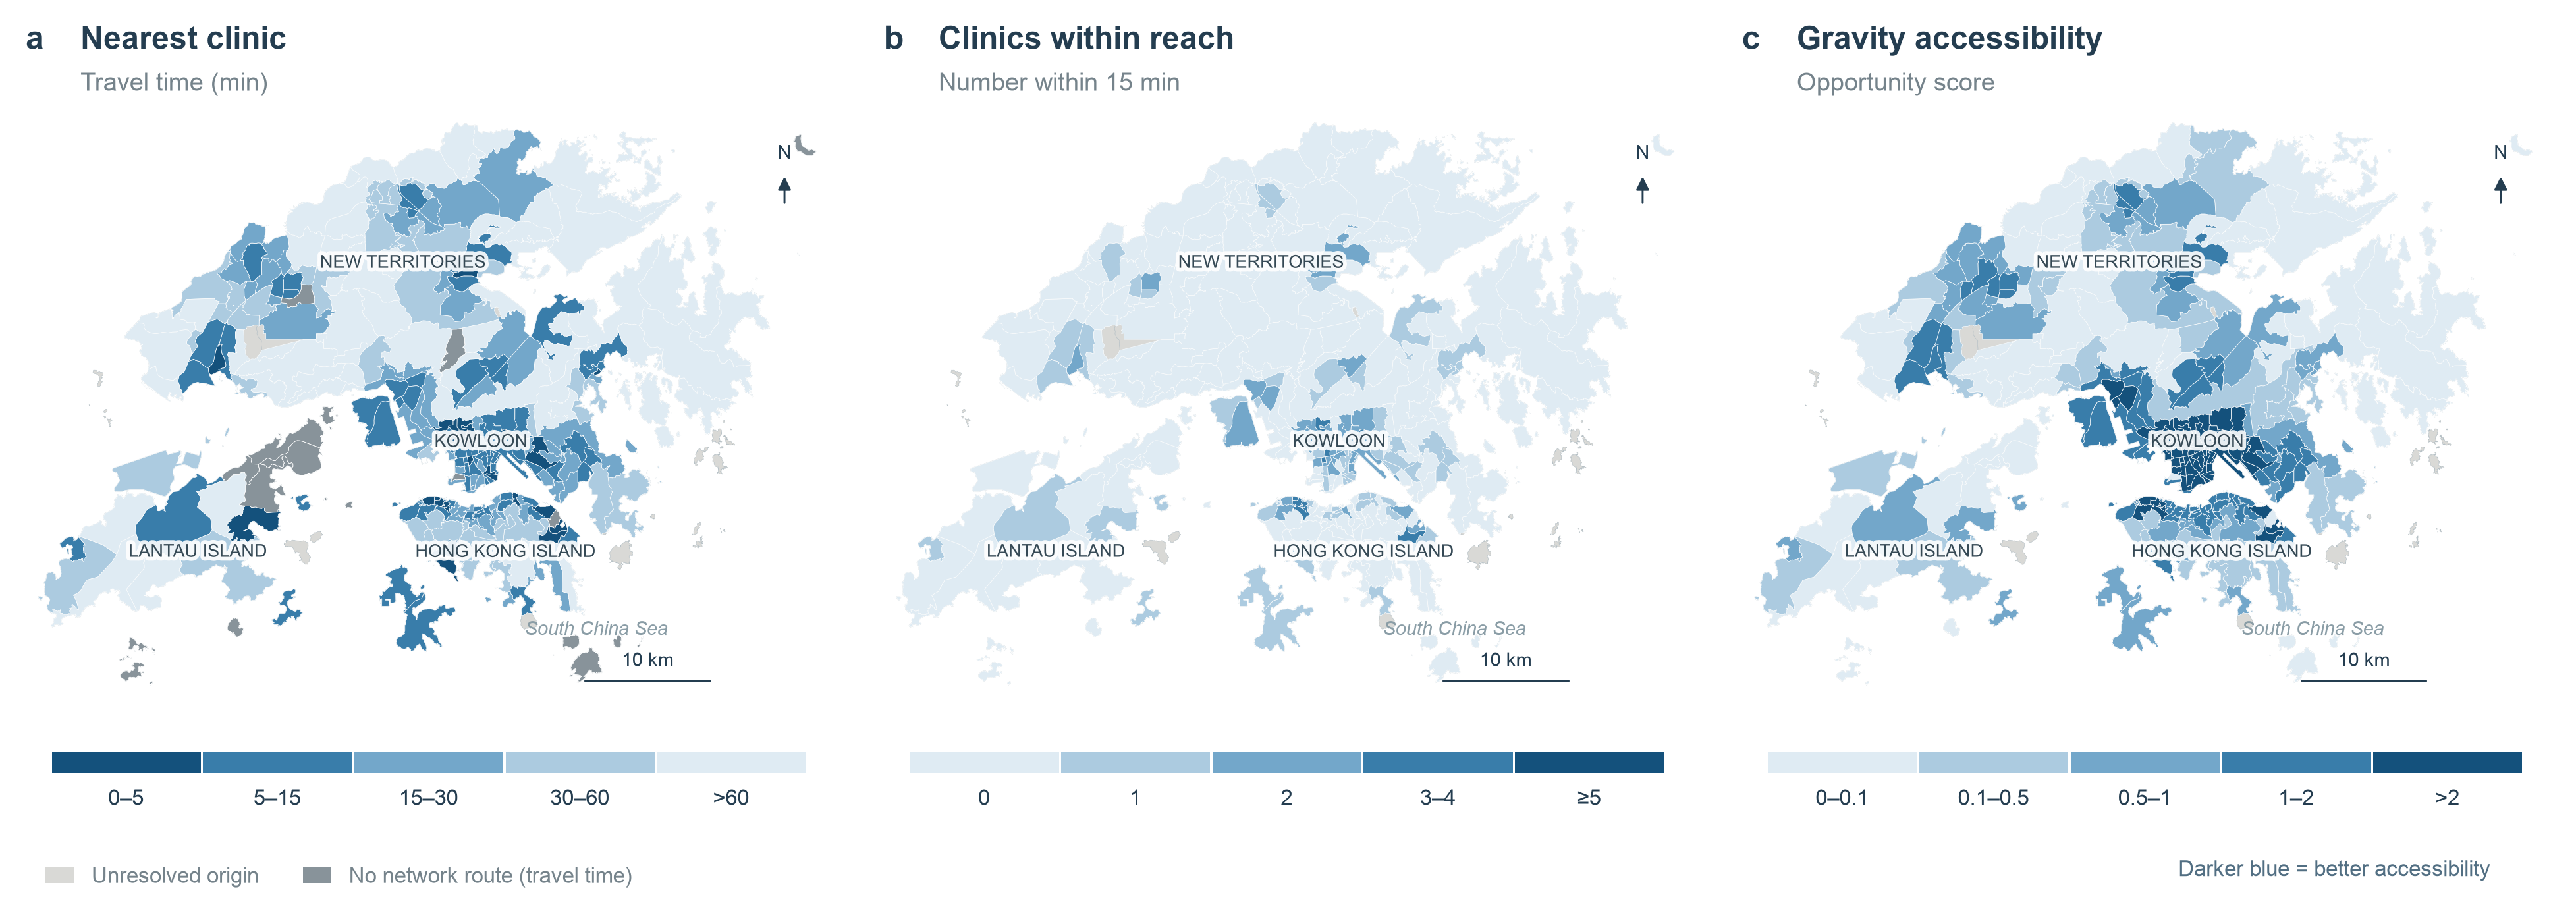
\includegraphics[width=0.92\linewidth,height=0.32\textheight,keepaspectratio]{accessibility_maps.png}
\caption{\textbf{Spatial variation in walking access to public primary care.} TPU proxy estimates of (a) $M$, (b) $C$ and (c) $G$. Darker blue indicates better access; light grey denotes unresolved origins and slate grey denotes no route in (a), with zero scores in (b,c). EPSG:2326. Data: CSDI~\cite{csdiClinics,csdiTPU,csdiCensus,csdiNetwork}.}
\label{fig:1}
\end{figure}

\begin{multicols}{2}
Spearman correlations were 0.848 for $-M$ versus $C$, 0.863 for $-M$ versus $G$, and 0.733 for $C$ versus $G$. Retaining tied zeros expanded $C$'s lowest-quintile set to 172 origins, compared with 57 each for $M$ and $G$. Jaccard overlap was 0.331 for either comparison involving $C$, versus 0.900 between $M$ and $G$.

TPUs 271, 236 and 291 had $C=0$, but nearest-clinic times were 19.03, 18.43 and 15.10 minutes and gravity scores 3.62, 3.40 and 3.10 (Figure~\ref{fig:2}a). They had three, five and five clinics within 30 minutes, respectively. Cutoffs of 10 and 30 minutes yielded 208 and 114 zero-opportunity origins, compared with 172 at 15 minutes.

\textbf{Slower walking reduces access despite stable rankings.}
At the slower speed, 43 additional origins had no clinic within 15 minutes. Gravity rankings remained strongly correlated with the baseline ($\rho=0.981$), although individual scores fell by a median of 56.3\% among origins with positive baseline scores (Figure~\ref{fig:2}b).
\end{multicols}

\begin{figure}[H]
\centering
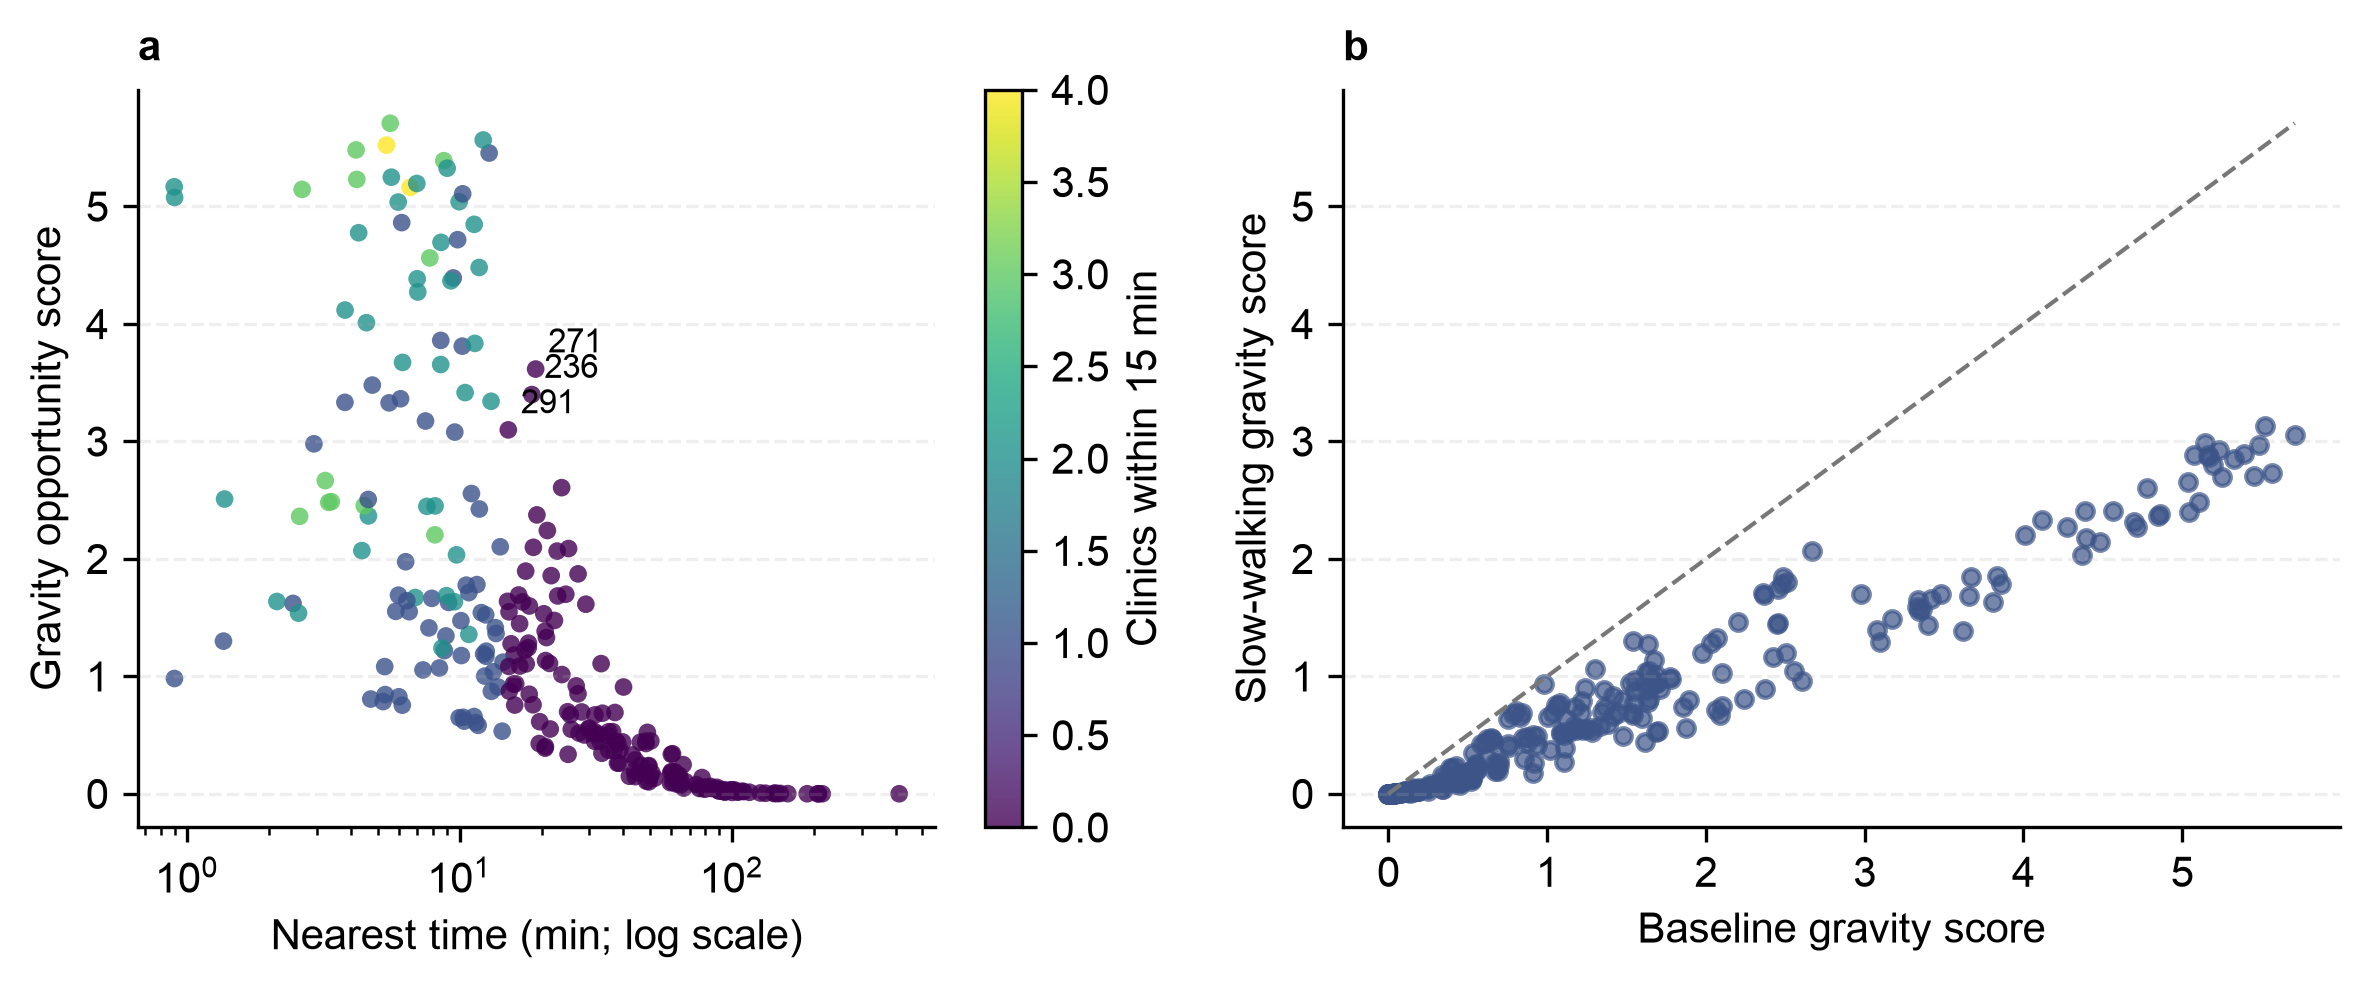
\includegraphics[width=0.92\linewidth,height=0.32\textheight,keepaspectratio]{figures/comparison.png}
\caption{\textbf{Indicator differences and walking-speed sensitivity.} Reachable origins: (a) $G$ versus $M$ (logarithmic axis), coloured by $C$; labels identify disagreement cases. (b) Gravity scores at 3.0 versus 4.8~km\,h$^{-1}$; the dashed line denotes equality.}
\label{fig:2}
\end{figure}

\clearpage
\begin{multicols}{2}
\section*{Discussion}
Minimum travel time describes the journey to the closest clinic, while cumulative opportunities summarise nearby choice. Gravity accessibility also accounts for more distant clinics, but the decay assumption influences its magnitude. Increasing the half-life from 10 to 20 minutes raised median gravity accessibility from 0.50 to 1.24.

Equal clinic weights leave capacity and competing population demand unaccounted for~\cite{xiong2022}. Entrances, network connections and lift waits affect journeys through Hong Kong's multilevel pedestrian environment. Figures~\ref{fig:3}--\ref{fig:4} support geometric inspection of the modelled connections. Using alternative origins changed whether $C=0$ in 34 of 206 tested TPUs. Within each scenario, a common speed overlooks differences in walking ability.

\section*{Extending accessibility to walking burden}
A burden-adjusted measure would replace travel time with least generalised route cost:
\[
G_i^*=\sum_j\exp[-(\ln2)c_{ij}^*/15].
\]
Here, $c_{ij}^*$ is the minimum route cost under person-specific speeds and route-condition penalties, with separate lift costs. In illustrative scenarios, penalties of 25\% and 50\% on uncovered walking edges left 12 and 28 additional origins without opportunities within 15 minute-equivalents of generalised cost. Calibration requires observed journeys and route conditions; clinic capacity and compatible population demand would support competition-adjusted estimates~\cite{xiong2022,geurs2004}.
\section*{Conclusion}
Fifteen-minute counts conceal differences in walking access to public primary care. Gravity-based accessibility is most informative about potential clinic choice in this study; minimum travel time describes the journey to the nearest clinic. Interpreting both alongside walking-speed sensitivity reveals differences among locations assigned the same threshold classification.
\small
\begin{thebibliography}{9}
\bibitem{moreno2021}
Moreno, C., Allam, Z., Chabaud, D., Gall, C. \& Pratlong, F. Introducing the ``15-Minute City'': Sustainability, Resilience and Place Identity in Future Post-Pandemic Cities. \textit{Smart Cities} \textbf{4}(1), 93--111 (2021). \url{https://doi.org/10.3390/smartcities4010006}

\bibitem{tomasiello2023}
Tomasiello, D. B., Herszenhut, D., Oliveira, J. L. A., Braga, C. K. V. \& Pereira, R. H. M. A time interval metric for cumulative opportunity accessibility. \textit{Applied Geography} \textbf{157}, 103007 (2023). \url{https://doi.org/10.1016/j.apgeog.2023.103007}

\bibitem{xiong2022}
Xiong, X., Li, V. J., Huang, B. \& Huo, Z. Equality and social determinants of spatial accessibility, availability, and affordability to primary health care in Hong Kong, a descriptive study from the perspective of spatial analysis. \textit{BMC Health Services Research} \textbf{22}, 1364 (2022). \url{https://doi.org/10.1186/s12913-022-08760-2}

\bibitem{geurs2004}
Geurs, K. T. \& van Wee, B. Accessibility evaluation of land-use and transport strategies: review and research directions. \textit{Journal of Transport Geography} \textbf{12}(2), 127--140 (2004). \url{https://doi.org/10.1016/j.jtrangeo.2003.10.005}
\end{thebibliography}

\begingroup
\renewcommand{\refname}{Official data sources}
\begin{thebibliography}{9}
\setcounter{enumiv}{4}
\bibitem{csdiClinics}
Hospital Authority. Hospital Authority Family Medicine Clinic List. \textit{CSDI Portal}. Clinic coordinates and consultation hours; retrieved 24 October 2026. \url{https://portal.csdi.gov.hk/csdi-webpage/dataset/fhb_rcd_1637050485482_89683}

\bibitem{csdiTPU}
Planning Department. Boundaries of Tertiary Planning Units \& Subunits (for 2021 Population Census). \textit{CSDI Portal}. 2021 TPU boundaries; retrieved 24 October 2026. \url{https://portal.csdi.gov.hk/csdi-webpage/dataset/pland_rcd_1634022783366_65050}

\bibitem{csdiCensus}
Census and Statistics Department. 2021 Population Census (Statistics and Boundaries of Small Subunit Groups). \textit{CSDI Portal}. 2021 population statistics and boundaries used for origin selection; retrieved 24 October 2026. \url{https://portal.csdi.gov.hk/csdi-webpage/dataset/censtatd_rcd_1635933365202_19171}

\bibitem{csdiNetwork}
Lands Department. 3D Pedestrian Network. \textit{CSDI Portal}. Network geometry, direction, access schedules and cover attributes. Revision: 16 September 2026; retrieved 24 October 2026. \url{https://portal.csdi.gov.hk/csdi-webpage/dataset/landsd_rcd_1637222018065_52265}
\end{thebibliography}
\endgroup
\section*{Code availability and reproducibility}Python scripts, pinned dependencies, frozen inputs and validation instructions are available at \url{https://github.com/Claire0712/LSGI2802_Assignment2}. Quick check: \texttt{python reproduce.py verify}. The README documents environment setup and full network rerouting.

\section*{AI Declaration}
This report has used AI-assisted tools for language refinement, structural editing, and formatting support. All arguments, interpretations, data selection, and final academic judgments are the sole responsibility of the author.

\end{multicols}

% Appendix uses portrait A4 pages with 4-by-3 route panels.
\clearpage
\appendix
\setcounter{figure}{0}
\renewcommand{\thefigure}{A\arabic{figure}}
\section*{Appendix A: Route geometry checks}
These 23 routes document modelled geometry and connections between origin proxies and clinic network nodes.
\begin{figure}[H]
\centering
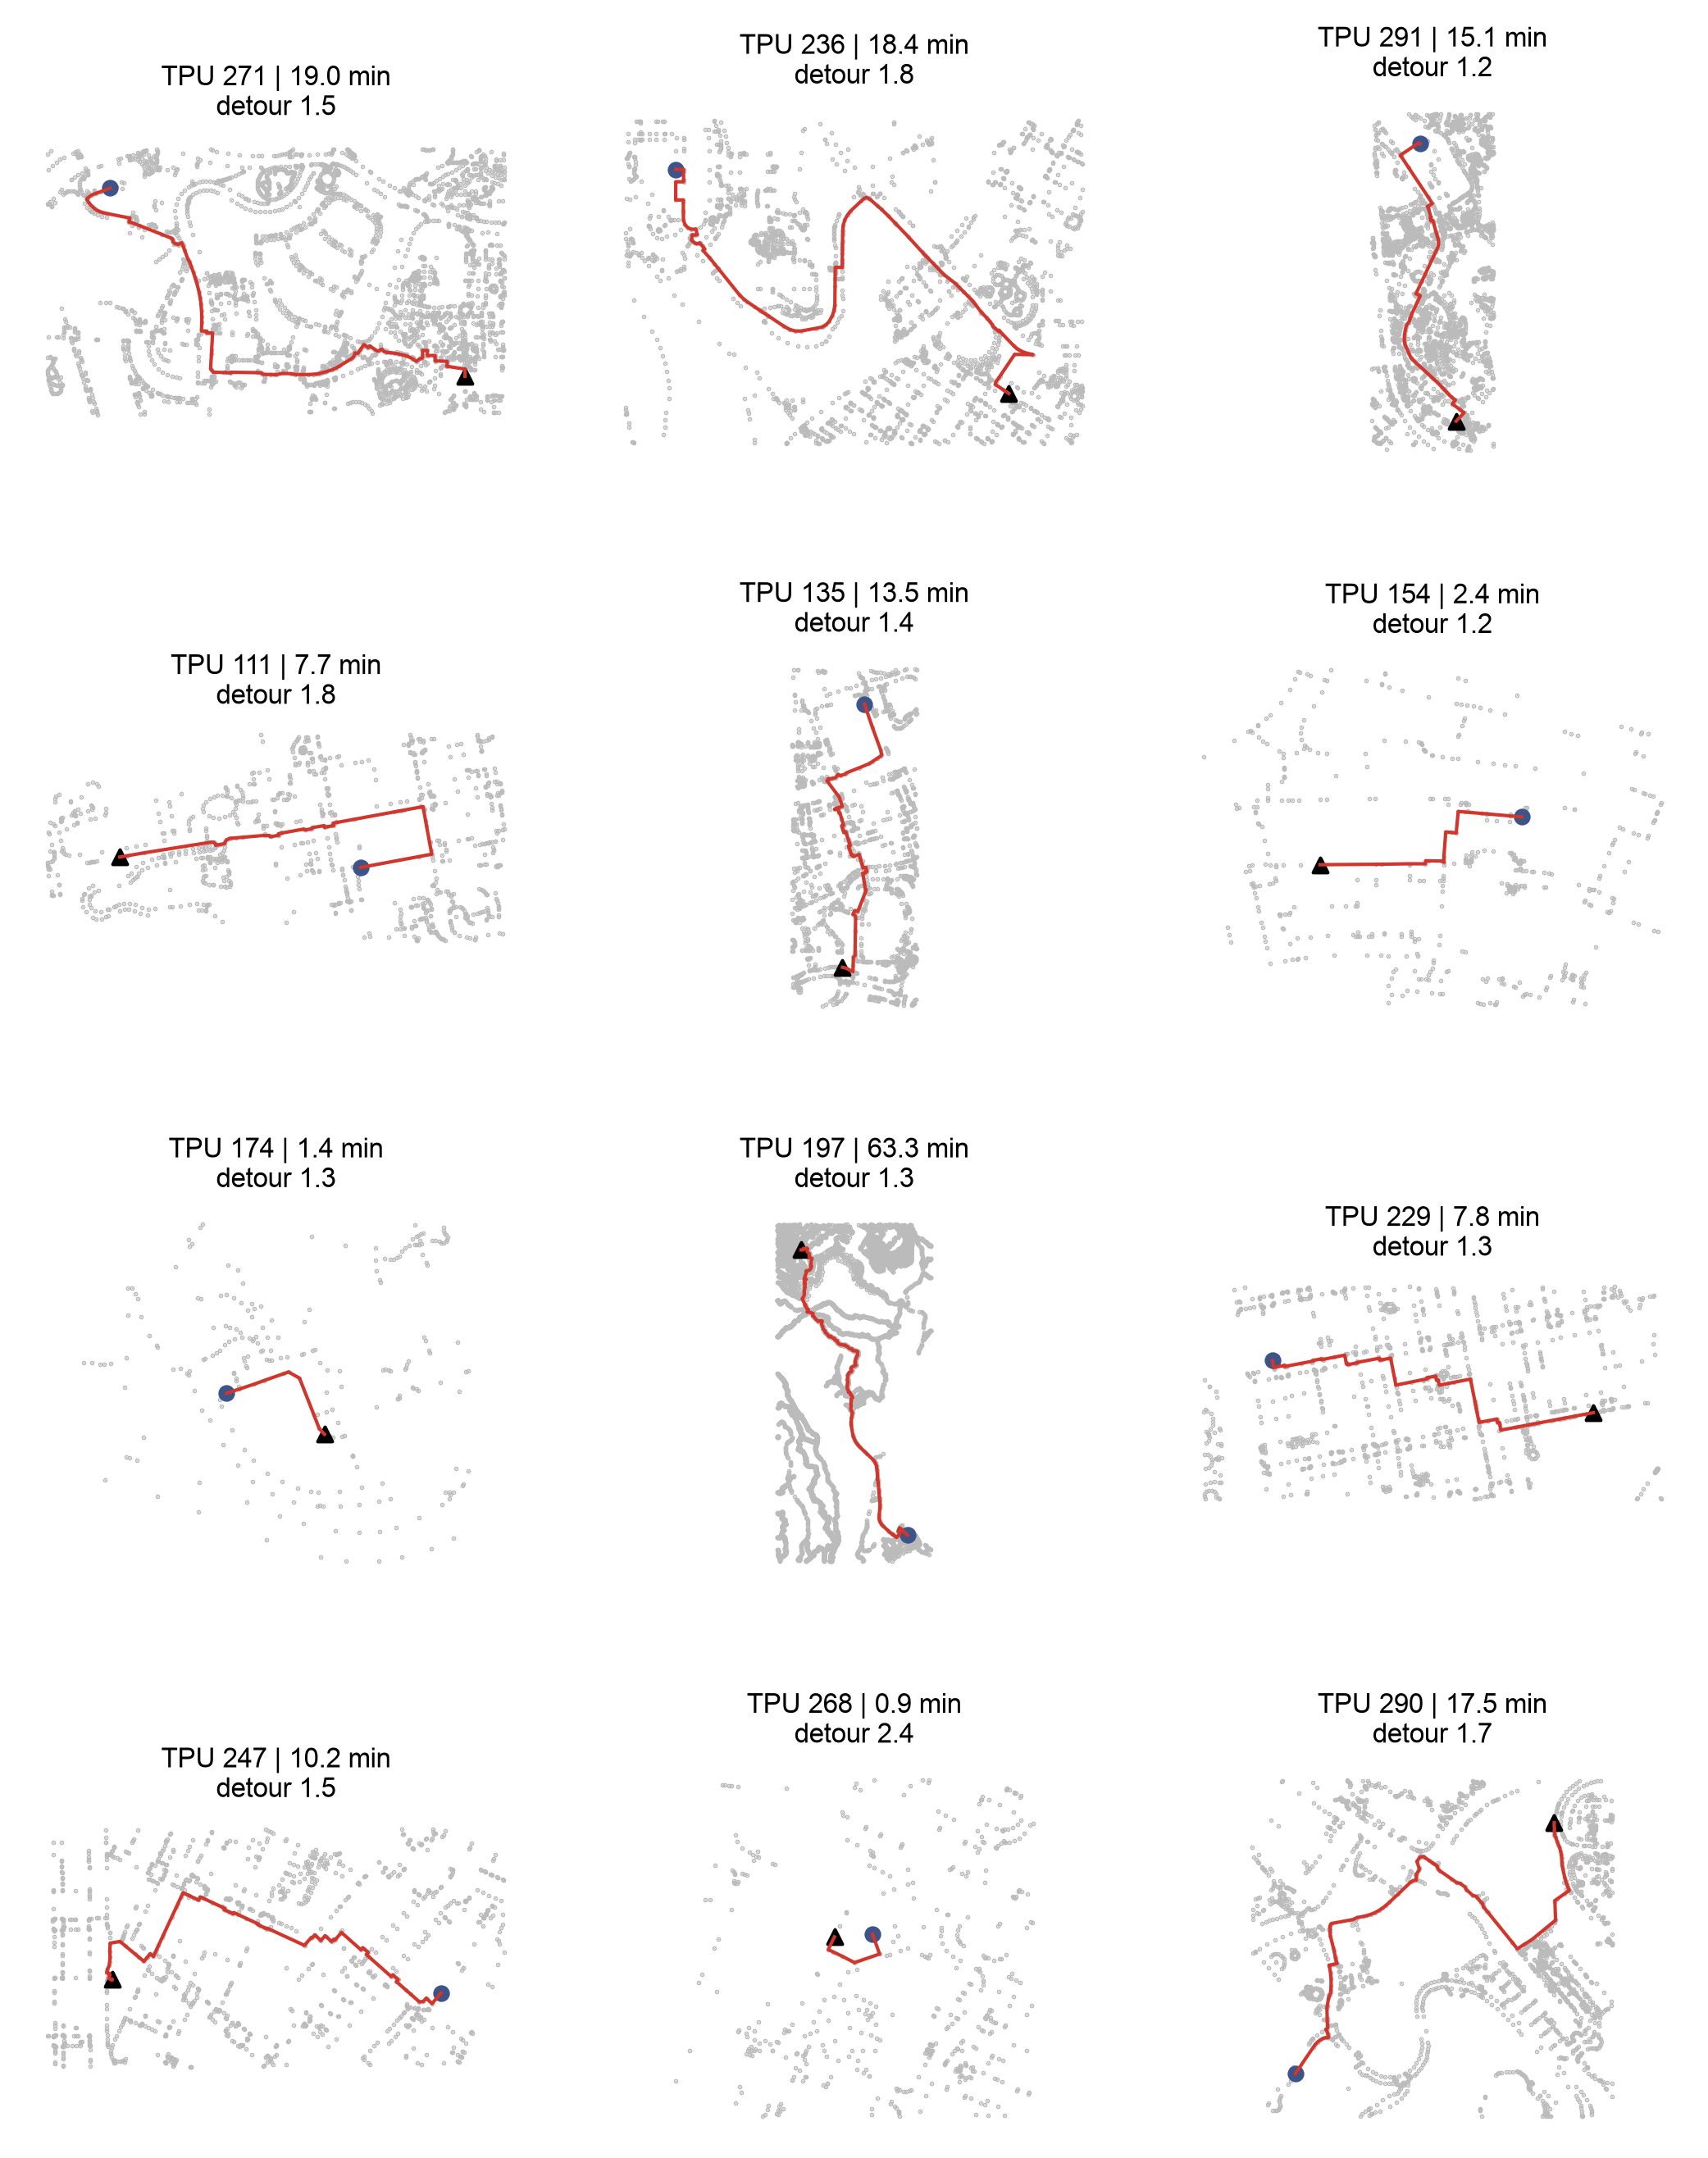
\includegraphics[width=\linewidth,height=0.83\textheight,keepaspectratio]{route_audit_portrait_page_1.png}
\caption{\textbf{Route geometry checks, cases 1--12.} Red: routes; blue: origins; triangles: destination nodes; grey: network vertices. Titles report TPU, travel time and route-to-straight-line distance ratio. Scales differ.}
\label{fig:3}
\end{figure}

\clearpage
\begin{figure}[H]
\centering
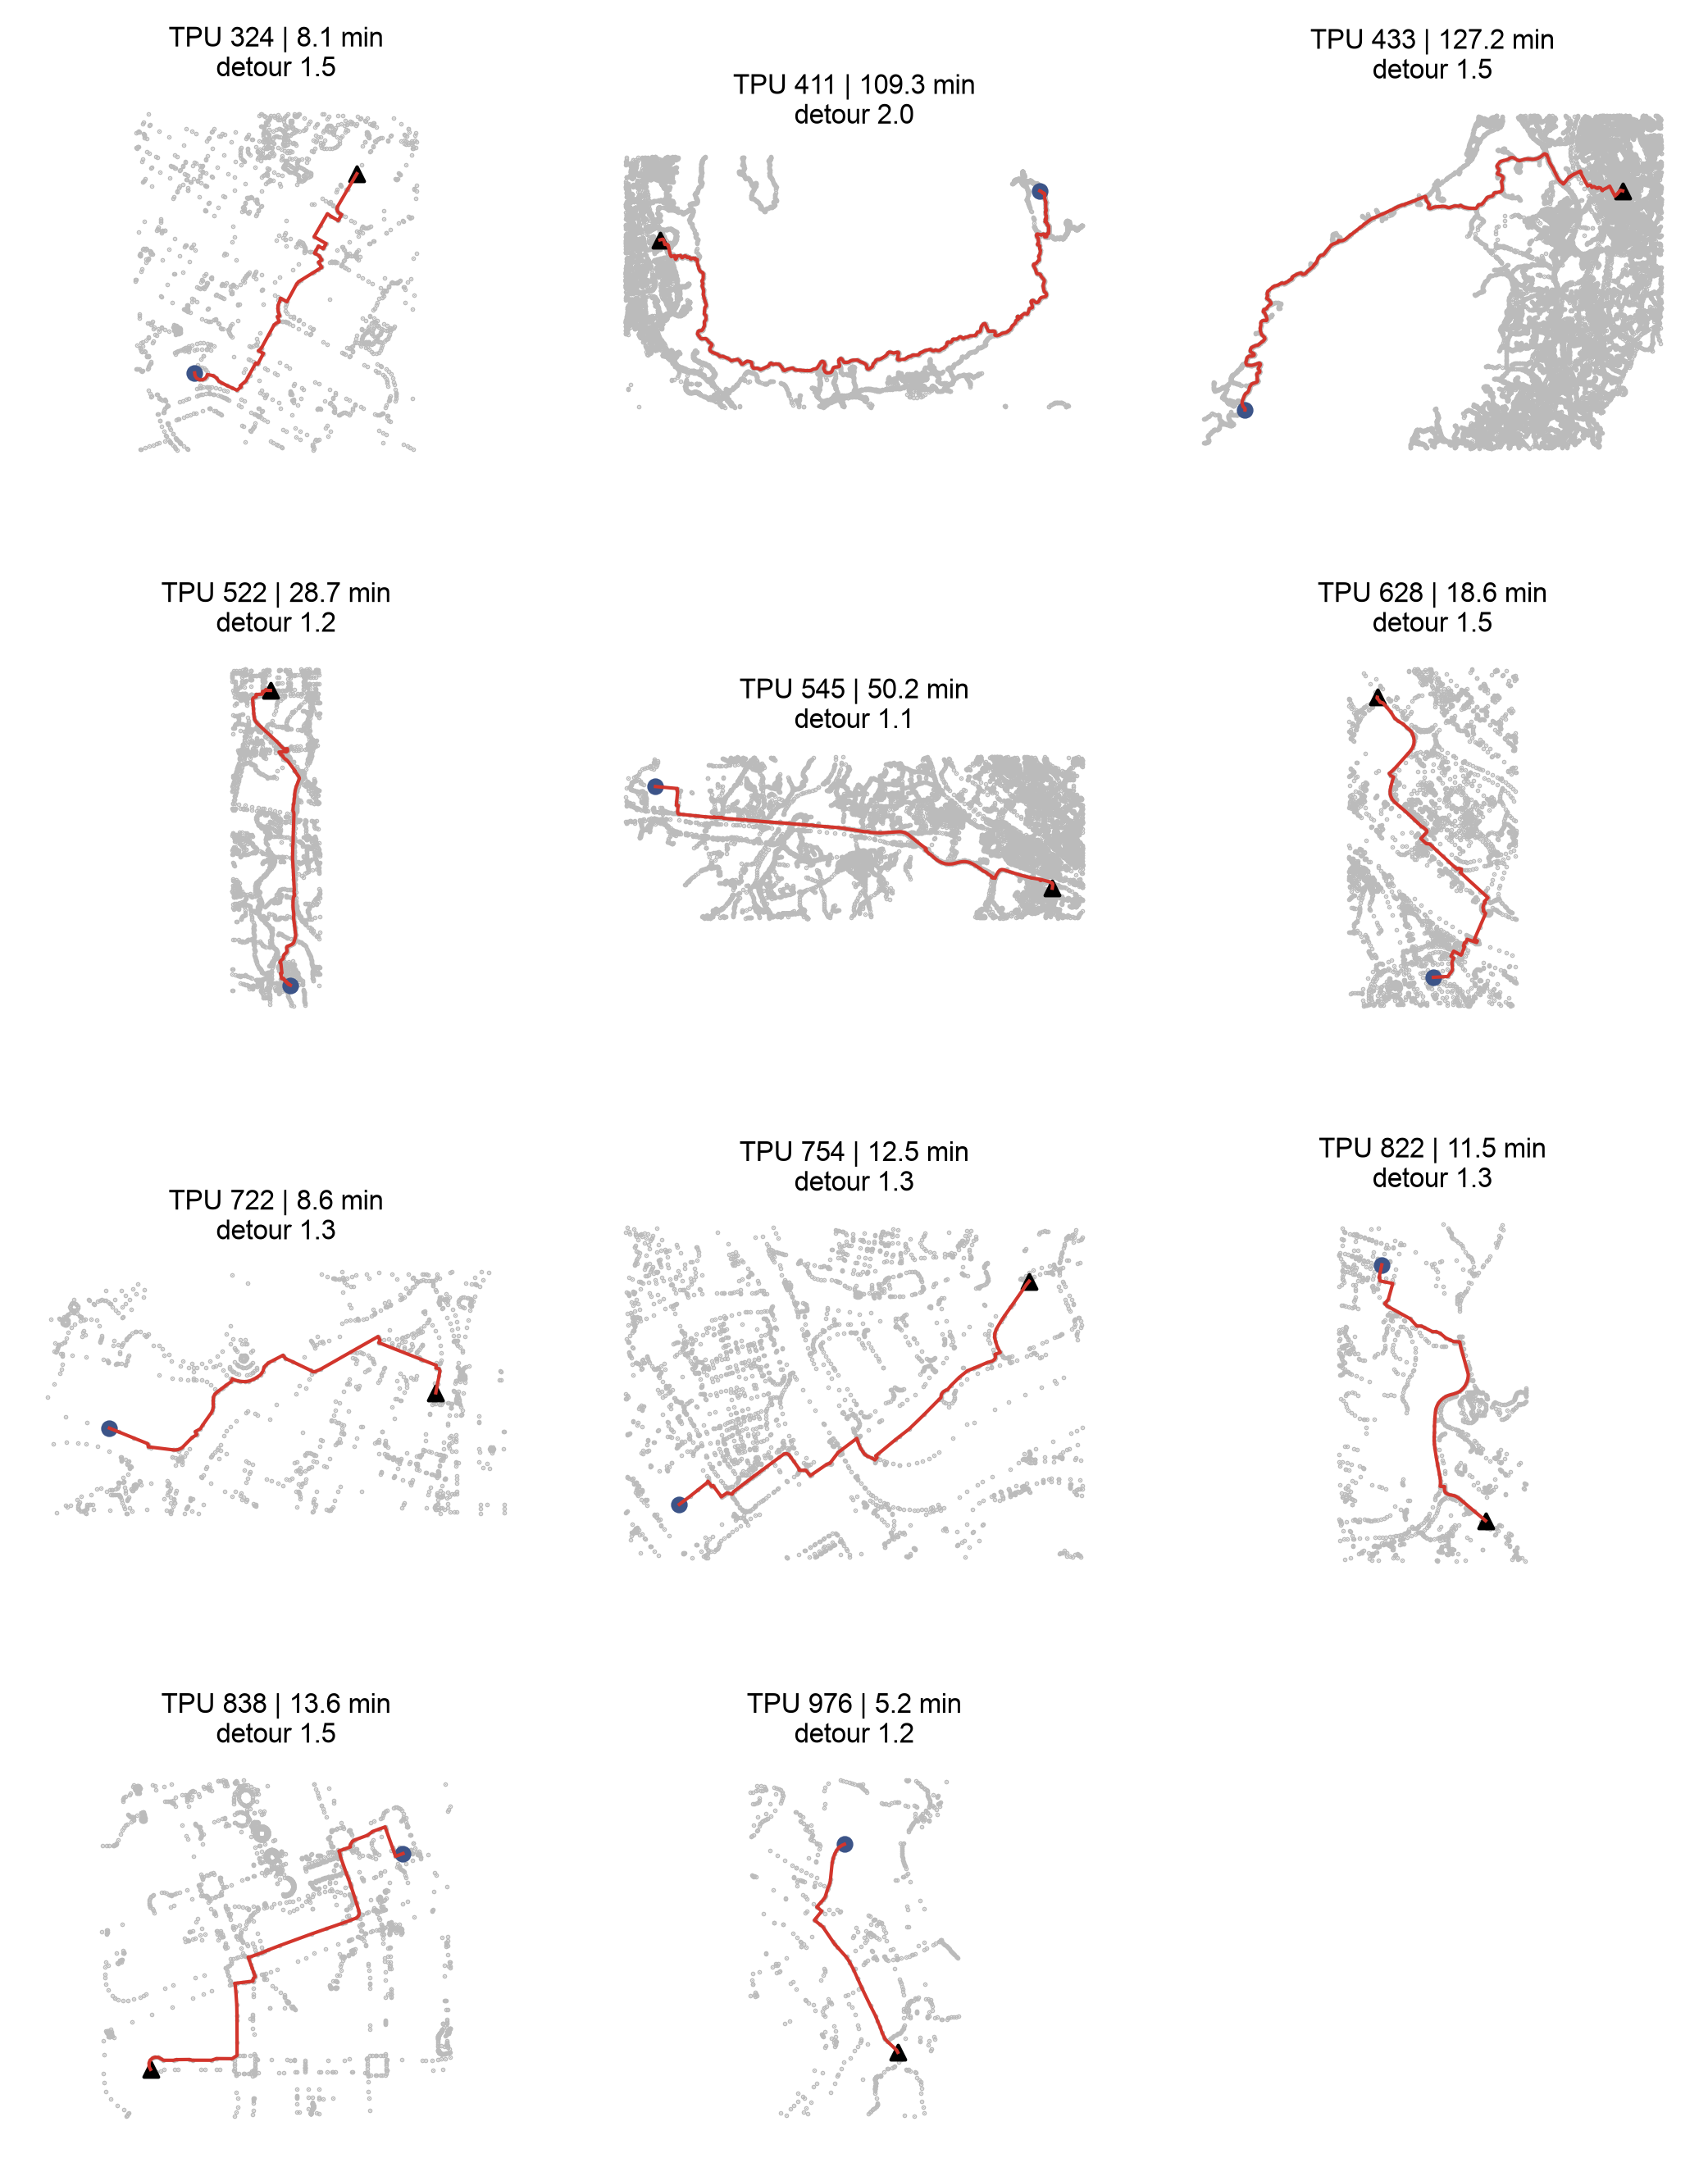
\includegraphics[width=\linewidth,height=0.83\textheight,keepaspectratio]{route_audit_portrait_page_2.png}
\caption{\textbf{Route geometry checks, cases 13--23.} Symbols and annotations follow Figure~\ref{fig:3}.}
\label{fig:4}
\end{figure}
\end{document}
